\begin{figure}[ht]
\centering
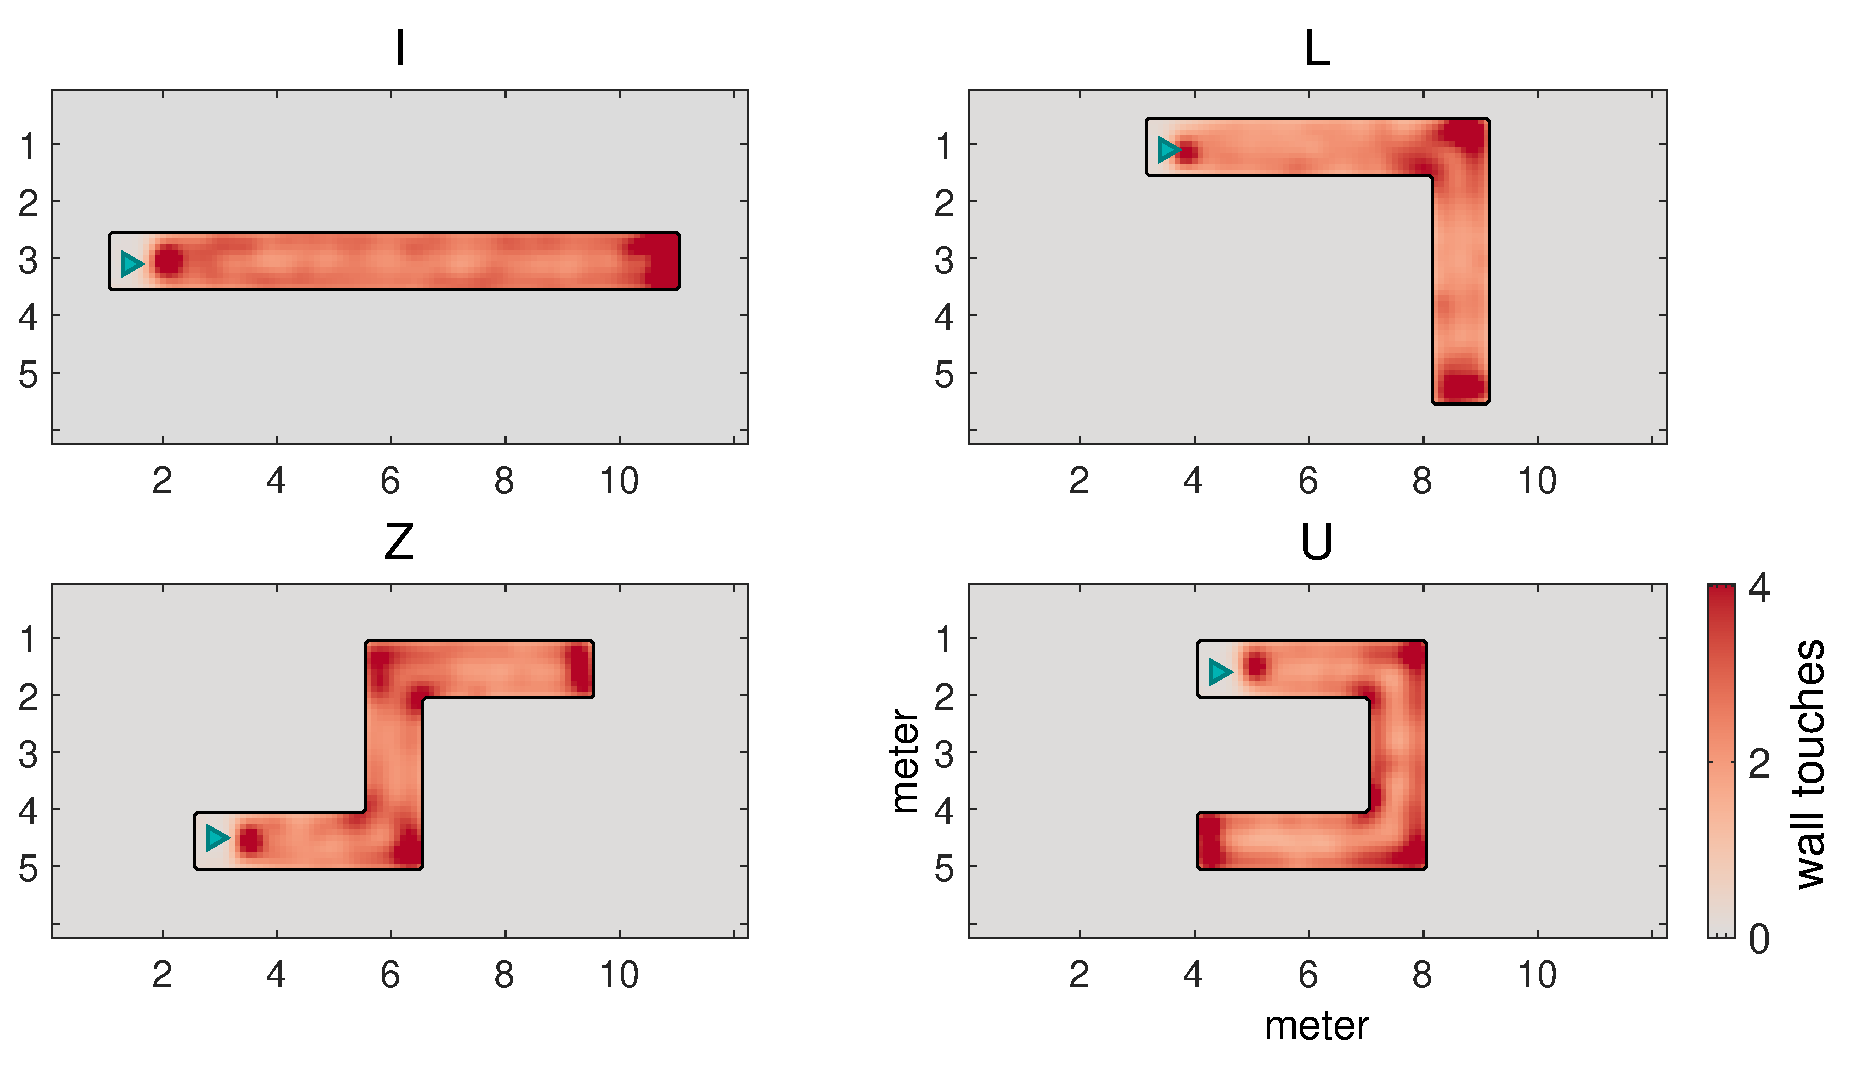
\includegraphics[width=\linewidth]{figures/duration_mean.eps}
\vspace{0pt}
\caption{Grand average duration in seconds spent at each location in each of the four different mazes: I, L, Z and U. The whole lab space is roughly 12 by 8 meters in size. Hotter colors, i.e. red, indicate a longer time spent at that location.}
\label{results_dur_mean}
\end{figure}

\subsection{Zooming in: Participants Exploration Behavior differs as a Function of Presence} First, we took a look at the grand average across participants for the two spatially resolved parameters 'time spent' as well as 'number of touches'. We observe a longer time spent at dead-ends as well as in the corners congruently across all mazes. On average participants spent about 4 second in each of hottest, i.e. reddest, locations in the corners and dead-ends, see figure \ref{results_dur_mean}. Participants spent less time when located in the straight segments of each maze, i.e. they moved faster in those segments. For the number of touches we observed a similar pattern, see figure \ref{results_touches_mean}. On average, participants touched the wall more frequent when located in the dead-ends and corners of the maze and exhihit less frequent wall touching along the straight segments. On average each pixel in the corners shows a likelihood of .08 that a wall was touched here.

\begin{figure}[h]
\centering
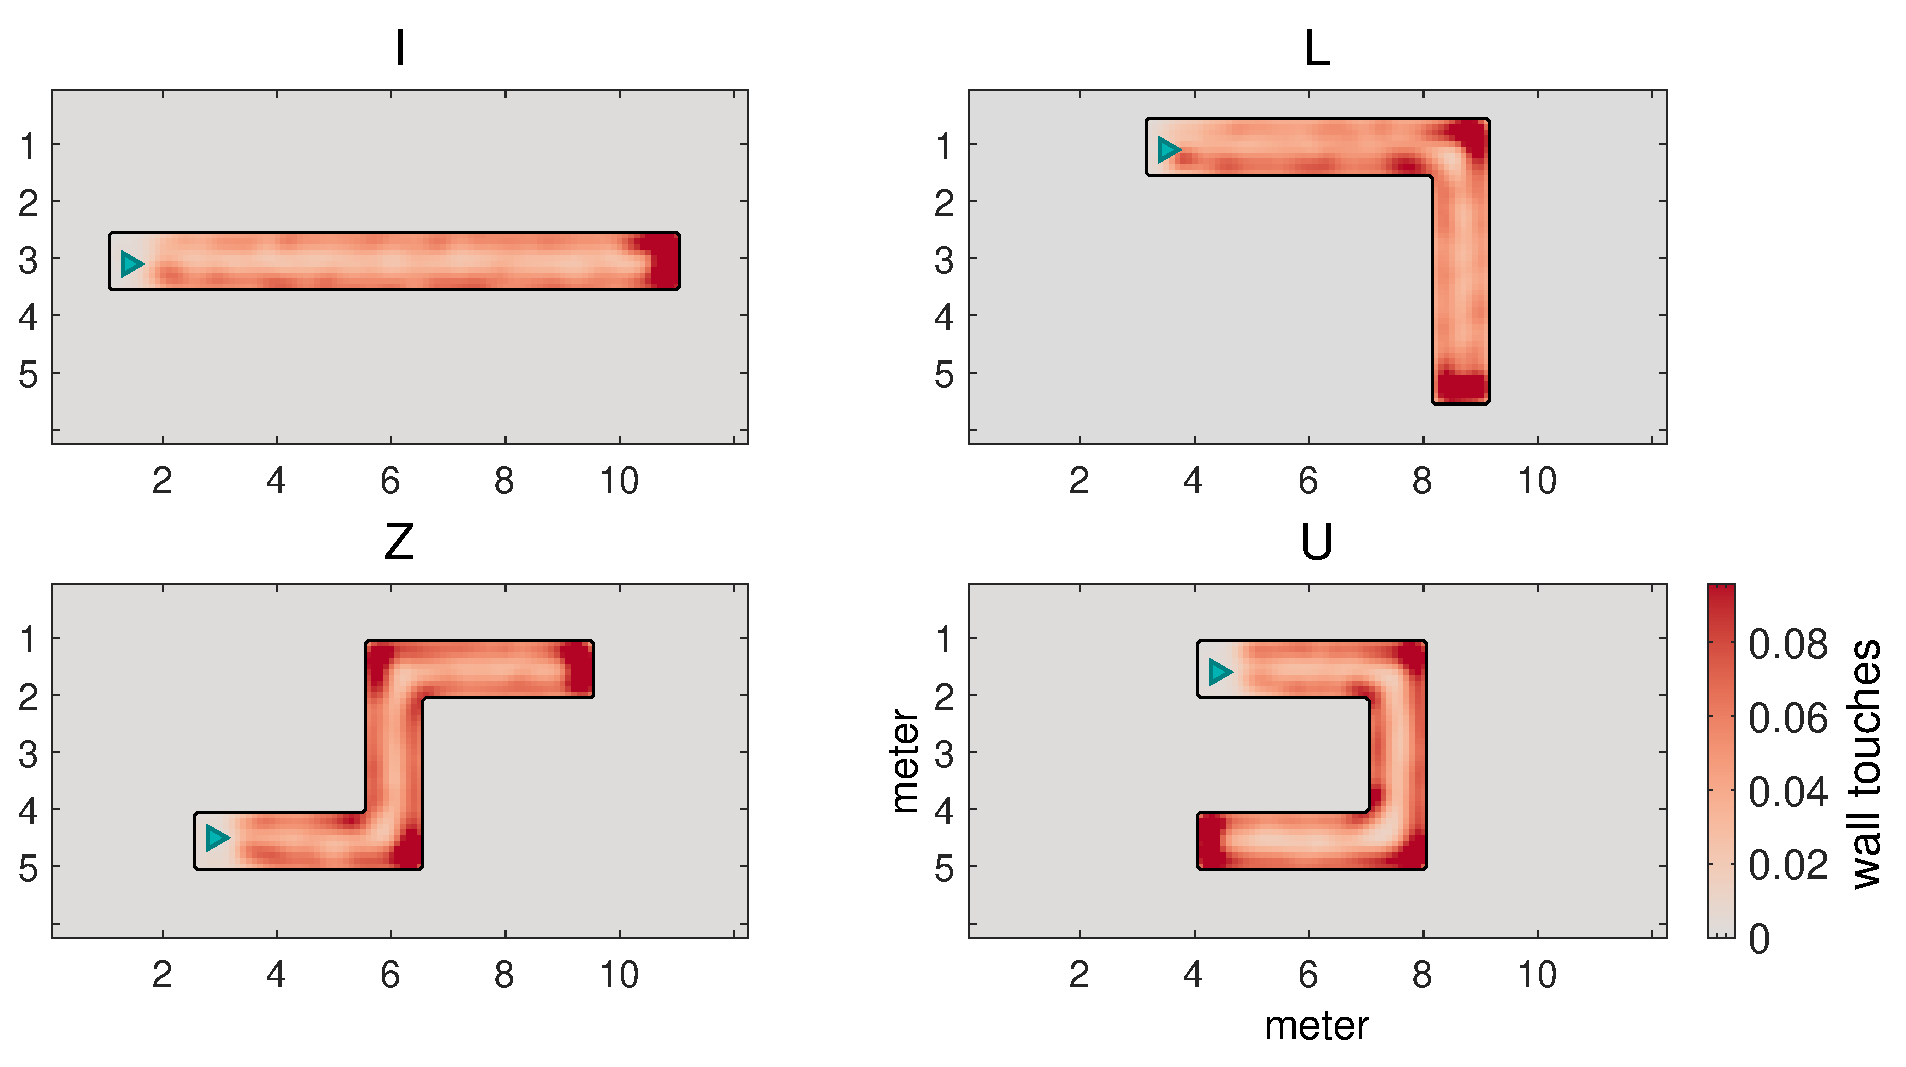
\includegraphics[width=\linewidth]{figures/wall_touches_mean.eps}
\vspace{0pt}
\caption{Grand average number of touches at each location in each of the four mazes: I, L, Z, U. Hotter colors, i.e. redder, indicate a higher number of touches. Note, the location of each wall touch was located to where the participants head (VR Headset) was located at that time point, not its hand.}
\label{results_touches_mean}
\end{figure}

Second, we investigated the effect of presence on time spent and number of touches at every location in all mazes. With increasing presence, we observed an increase in time spent at the corners and dead-ends of the mazes, see figure \ref{results_dur_effect}. Furthermore, with increasing presence a decrease in time spent at the center of the path, the paths were 1m wide, was observed for all mazes. Interestingly, this effect was significant for portions of the straight 'I' maze as well as the second straight segment of the 'Z' maze. For the 'L' maze we observed a significant effect of presence on the time spent in the center of the first turn. Similar significant locations were observed in the second turn of the 'U' maze. Taken together, with an increase in experienced presence, participants spent more time closer to the walls and less in the center of the paths. Additionally, this effect showed most prominent in the corners of the 'L', 'Z' and 'U' maze as well as along the straight of the 'I' and 'Z' maze.

\begin{figure}[h]
\centering
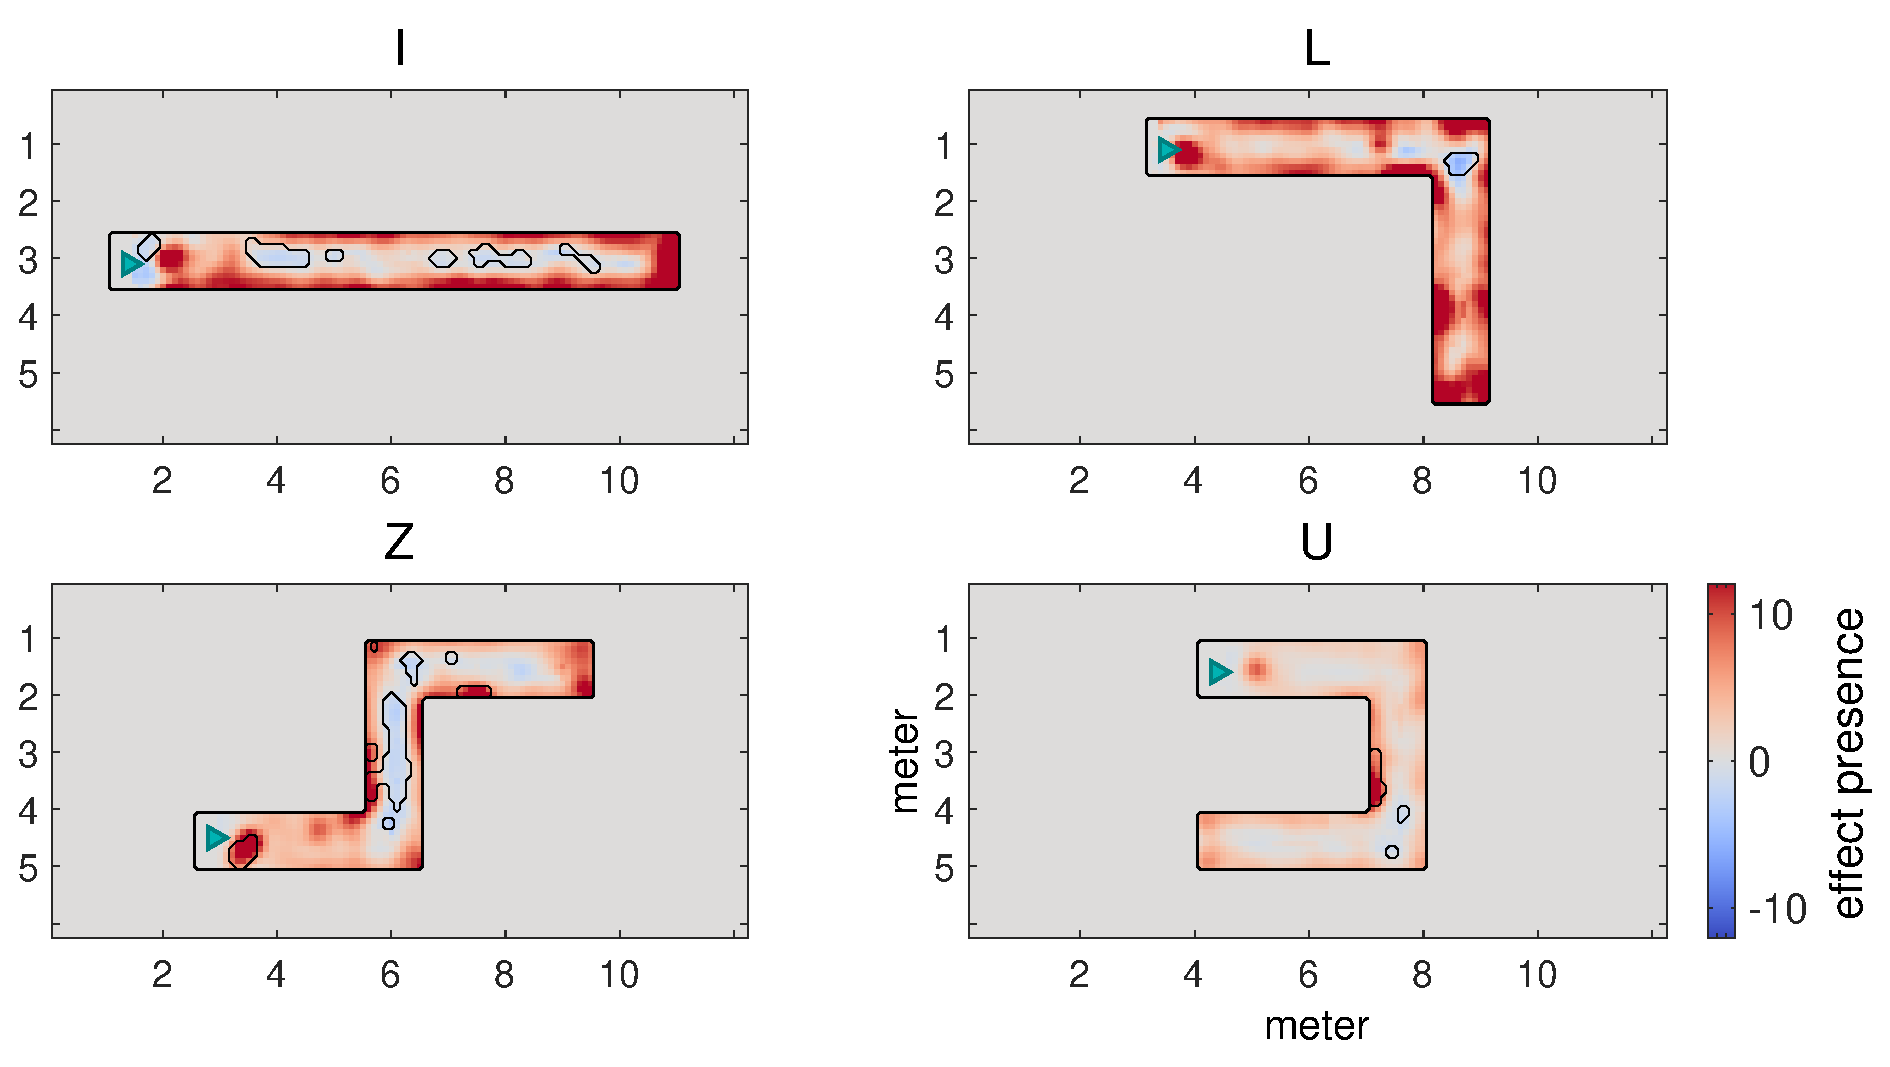
\includegraphics[width=\linewidth]{figures/effect_presence_duration.eps}
\vspace{0pt}
\caption{Map of the impact of presence on the time spent at every location in each of the four mazes: I, L, Z, U. Warmer colors refer to a positive regression estimate. For easy readability we introduce the reasoning for a positive estimate: for each 1 point increase in reported presence, participants stayed z seconds longer at location xy.}
\label{results_dur_effect}
\end{figure}

The effect of presence on the number of spatially resolved wall touches showed less spatial specificity. Participants with higher reported presence had overall more wall touches than participants with a lower score. Presence did not significantly impact the spatial distribution of wall touches during exploration. We did observe a positive effect of presence on the number of wall touches along inside corner and dead-ends of mazes 'L' and 'U'. Higher experienced presence coincided with an increase in the number of touches along those corners and dead-ends, see figure \ref{results_touches_effect}.

\begin{figure}[h]
\centering
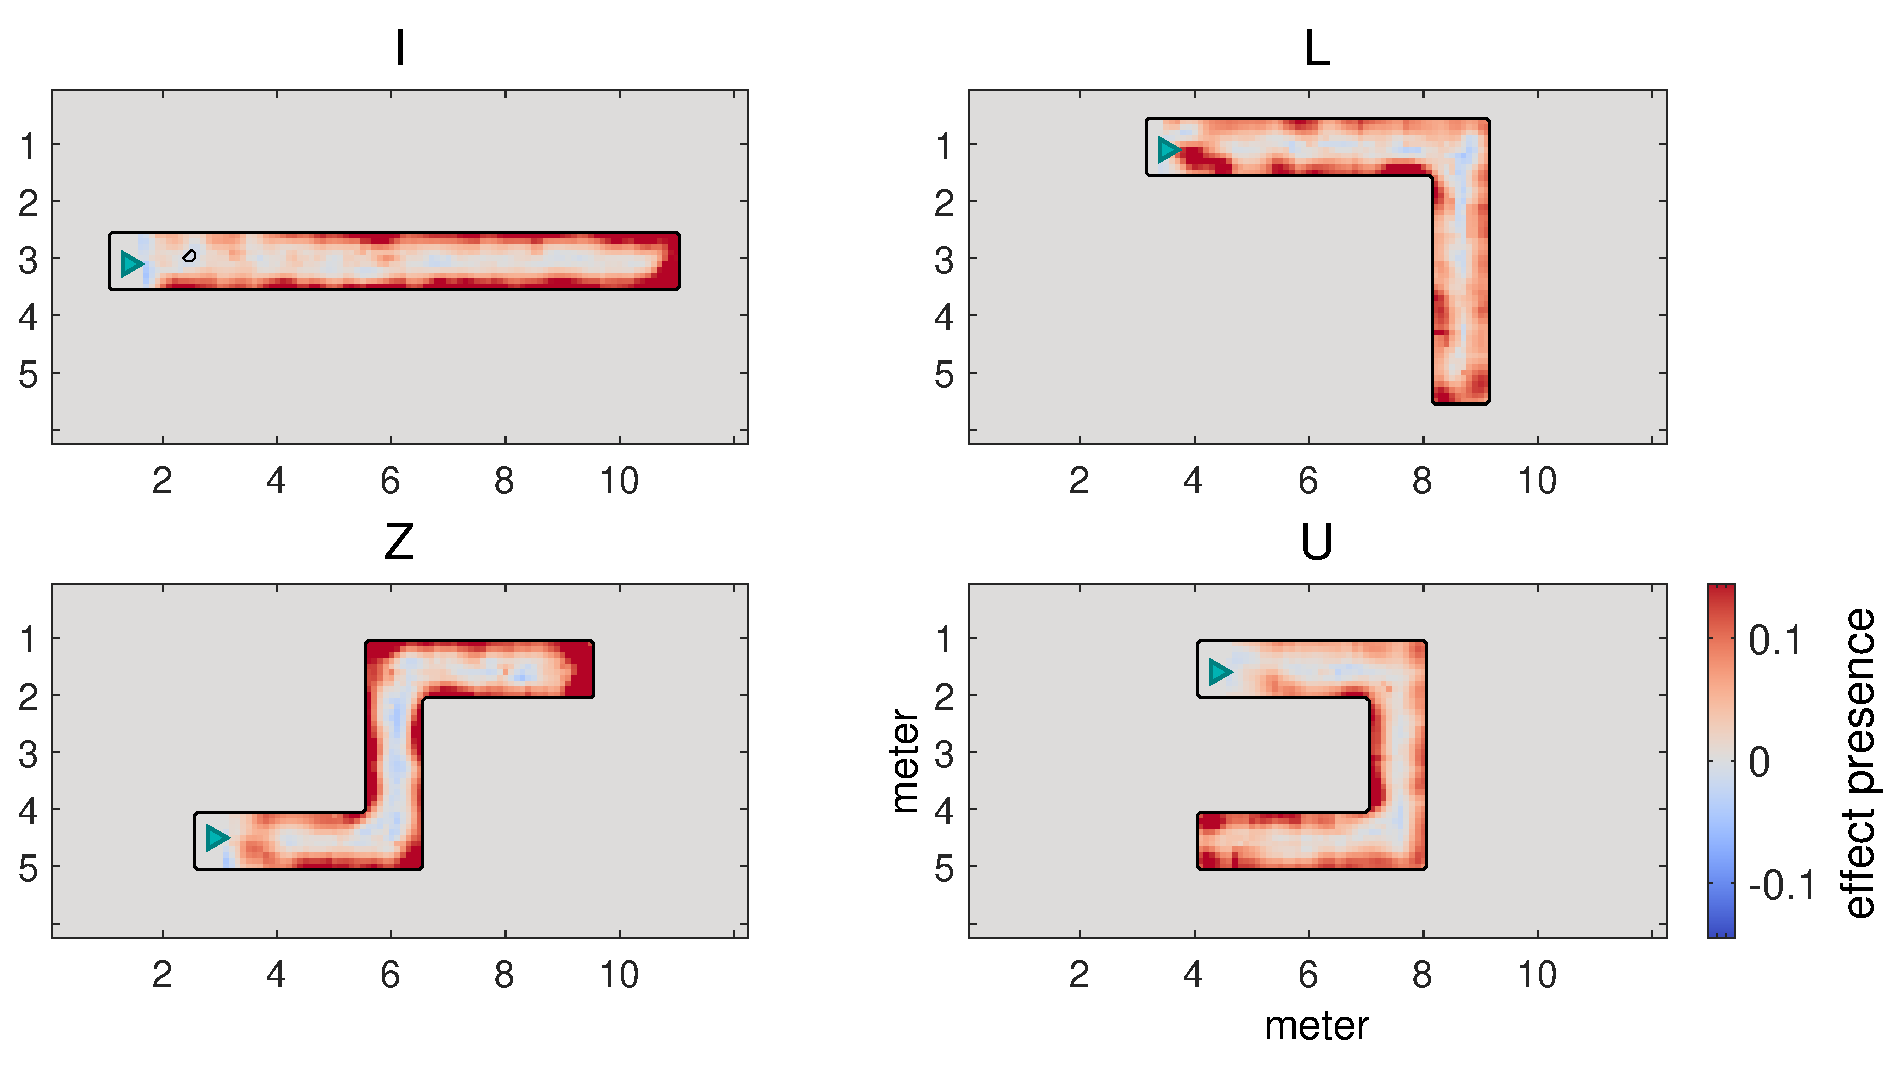
\includegraphics[width=\linewidth]{figures/effect_presence_wall_touches.eps}
\vspace{0pt}
\caption{{Map of the impact of presence on the number of touches at every location in each of the four mazes: I, L, Z, U. Warmer colors refer to a positive regression estimate. For easy readability we introduce the reasoning for a positive estimate: for each 1 point increase in reported presence, participants touched the walls z times at location xy.}}
\label{results_touches_effect}
\end{figure}